\documentclass[aspectratio=169]{beamer}
\usetheme{Madrid}
\usecolortheme{default}
\usepackage[utf8]{inputenc}
\usepackage[T5]{fontenc}
\usepackage{graphicx}
\usepackage{hyperref}
\usepackage{booktabs}
\usepackage{amsmath}
\usepackage{listings}
\usepackage{xcolor}

\setbeamertemplate{caption}[numbered]
\renewcommand{\figurename}{Hình}
\renewcommand{\thefigure}{13.\arabic{figure}}

\definecolor{codegreen}{rgb}{0,0.6,0}
\definecolor{codegray}{rgb}{0.5,0.5,0.5}
\definecolor{codepurple}{rgb}{0.58,0,0.82}
\definecolor{backcolour}{rgb}{0.95,0.95,0.92}

\lstset{
    backgroundcolor=\color{backcolour},   
    commentstyle=\color{codegreen},
    keywordstyle=\color{magenta},
    numberstyle=\tiny\color{codegray},
    stringstyle=\color{codepurple},
    basicstyle=\ttfamily\scriptsize,
    breakatwhitespace=false,         
    breaklines=true,                 
    captionpos=b,                    
    keepspaces=true,                 
    numbers=left,                    
    numbersep=5pt,                  
    showspaces=false,                
    showstringspaces=false,
    showtabs=false,                  
    tabsize=2
}

\title[Chương 13: Timeseries Forecasting]{Học Sâu (Deep Learning) \\ \vspace{0.5cm} \Large Chương 13: Dự báo Chuỗi thời gian \\ (Timeseries Forecasting)}
\author{Đại học Đông Á}
\date{\today}

\begin{document}

\begin{frame}
    \titlepage
\end{frame}

\begin{frame}{Nội dung chương}
    \tableofcontents
\end{frame}

\section{1. Giới thiệu Chuỗi thời gian và Bài toán Dự báo}

\begin{frame}{Chuỗi thời gian (Timeseries) là gì?}
    \begin{itemize}
        \item Chuỗi thời gian là tập hợp các điểm dữ liệu được ghi nhận theo những khoảng thời gian đều đặn.
        \item Yếu tố \textbf{"Thứ tự"} (Temporal Order) mang tính quyết định. Quá khứ ảnh hưởng đến tương lai.
        \item Bài toán phổ biến nhất: \textbf{Dự báo (Forecasting)} - Dự đoán điều gì sẽ xảy ra tiếp theo.
        \item Ứng dụng: Dự báo tiêu thụ điện năng, dự báo doanh thu, dự báo thời tiết, hoặc giao dịch chứng khoán.
    \end{itemize}
\end{frame}

\begin{frame}{Khảo sát Dữ liệu Thời tiết Jena (Dài hạn)}
    \begin{columns}
        \column{0.5\textwidth}
        \begin{itemize}
            \item Bộ dữ liệu từ Viện Max Planck, Đức. Ghi nhận 14 thông số thời tiết mỗi 10 phút.
            \item Trực quan hóa Biểu đồ Nhiệt độ trong khoảng thời gian nhiều năm.
            \item \textbf{Đặc điểm:} Có tính chu kỳ (Seasonality) rất rõ rệt theo các năm (Mùa đông lạnh, mùa hè nóng).
        \end{itemize}
        
        \column{0.5\textwidth}
        \begin{figure}
            \centering
            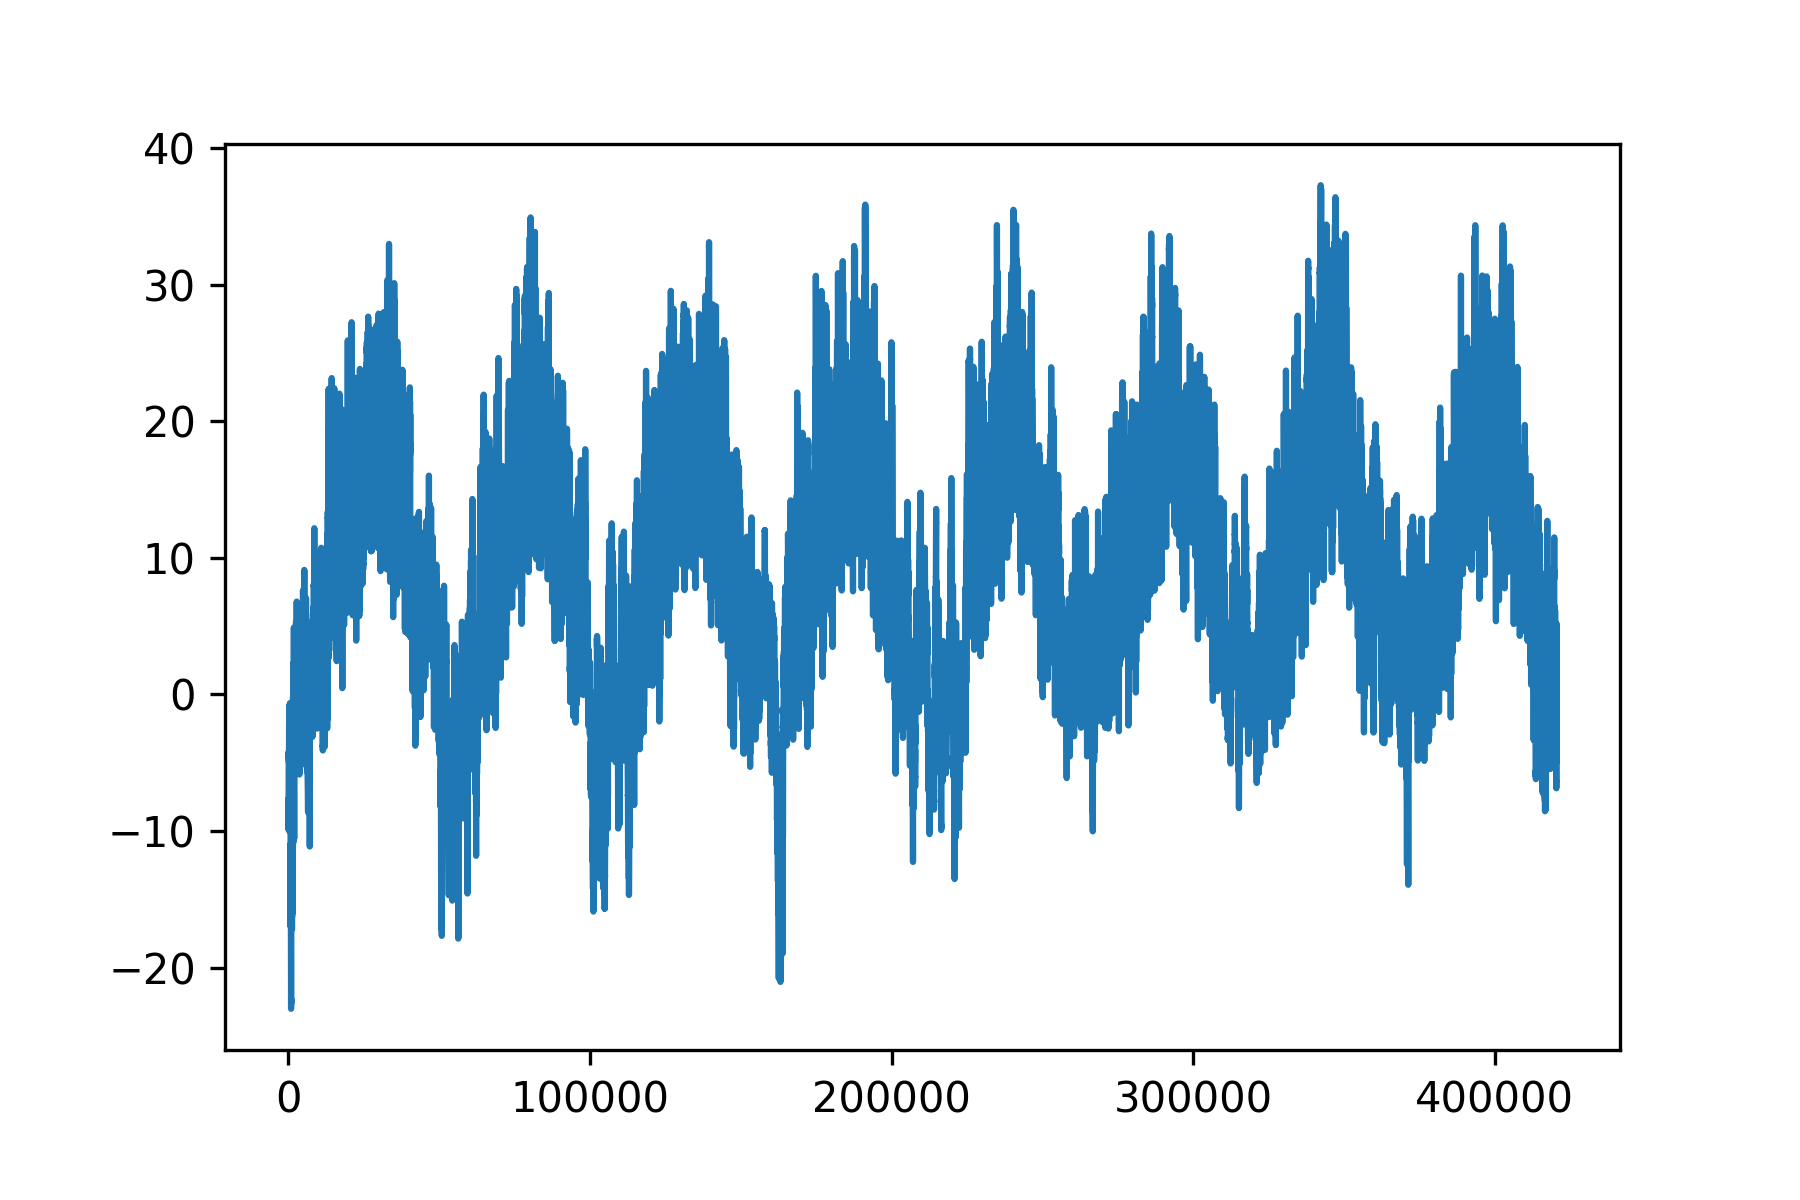
\includegraphics[width=\textwidth,height=0.6\textheight,keepaspectratio]{../../images/ch13/temperature_over_several_years.365f2e2e.png}
            \caption{Nhiệt độ thay đổi qua nhiều năm}
        \end{figure}
    \end{columns}
\end{frame}

\begin{frame}{Khảo sát Dữ liệu Thời tiết Jena (Ngắn hạn)}
    \begin{columns}
        \column{0.5\textwidth}
        \begin{itemize}
            \item Trực quan hóa chi tiết trong vòng 10 ngày (1440 điểm dữ liệu đầu tiên).
            \item Vẫn quan sát được tính chu kỳ theo ngày (Ngày ấm, đêm lạnh).
            \item Tuy nhiên, dữ liệu rất nhiễu và biến động mạnh do các yếu tố ngẫu nhiên.
            \item \textbf{Mục tiêu:} Dựa vào dữ liệu quá khứ, dự báo nhiệt độ của 24 giờ tiếp theo.
        \end{itemize}
        
        \column{0.5\textwidth}
        \begin{figure}
            \centering
            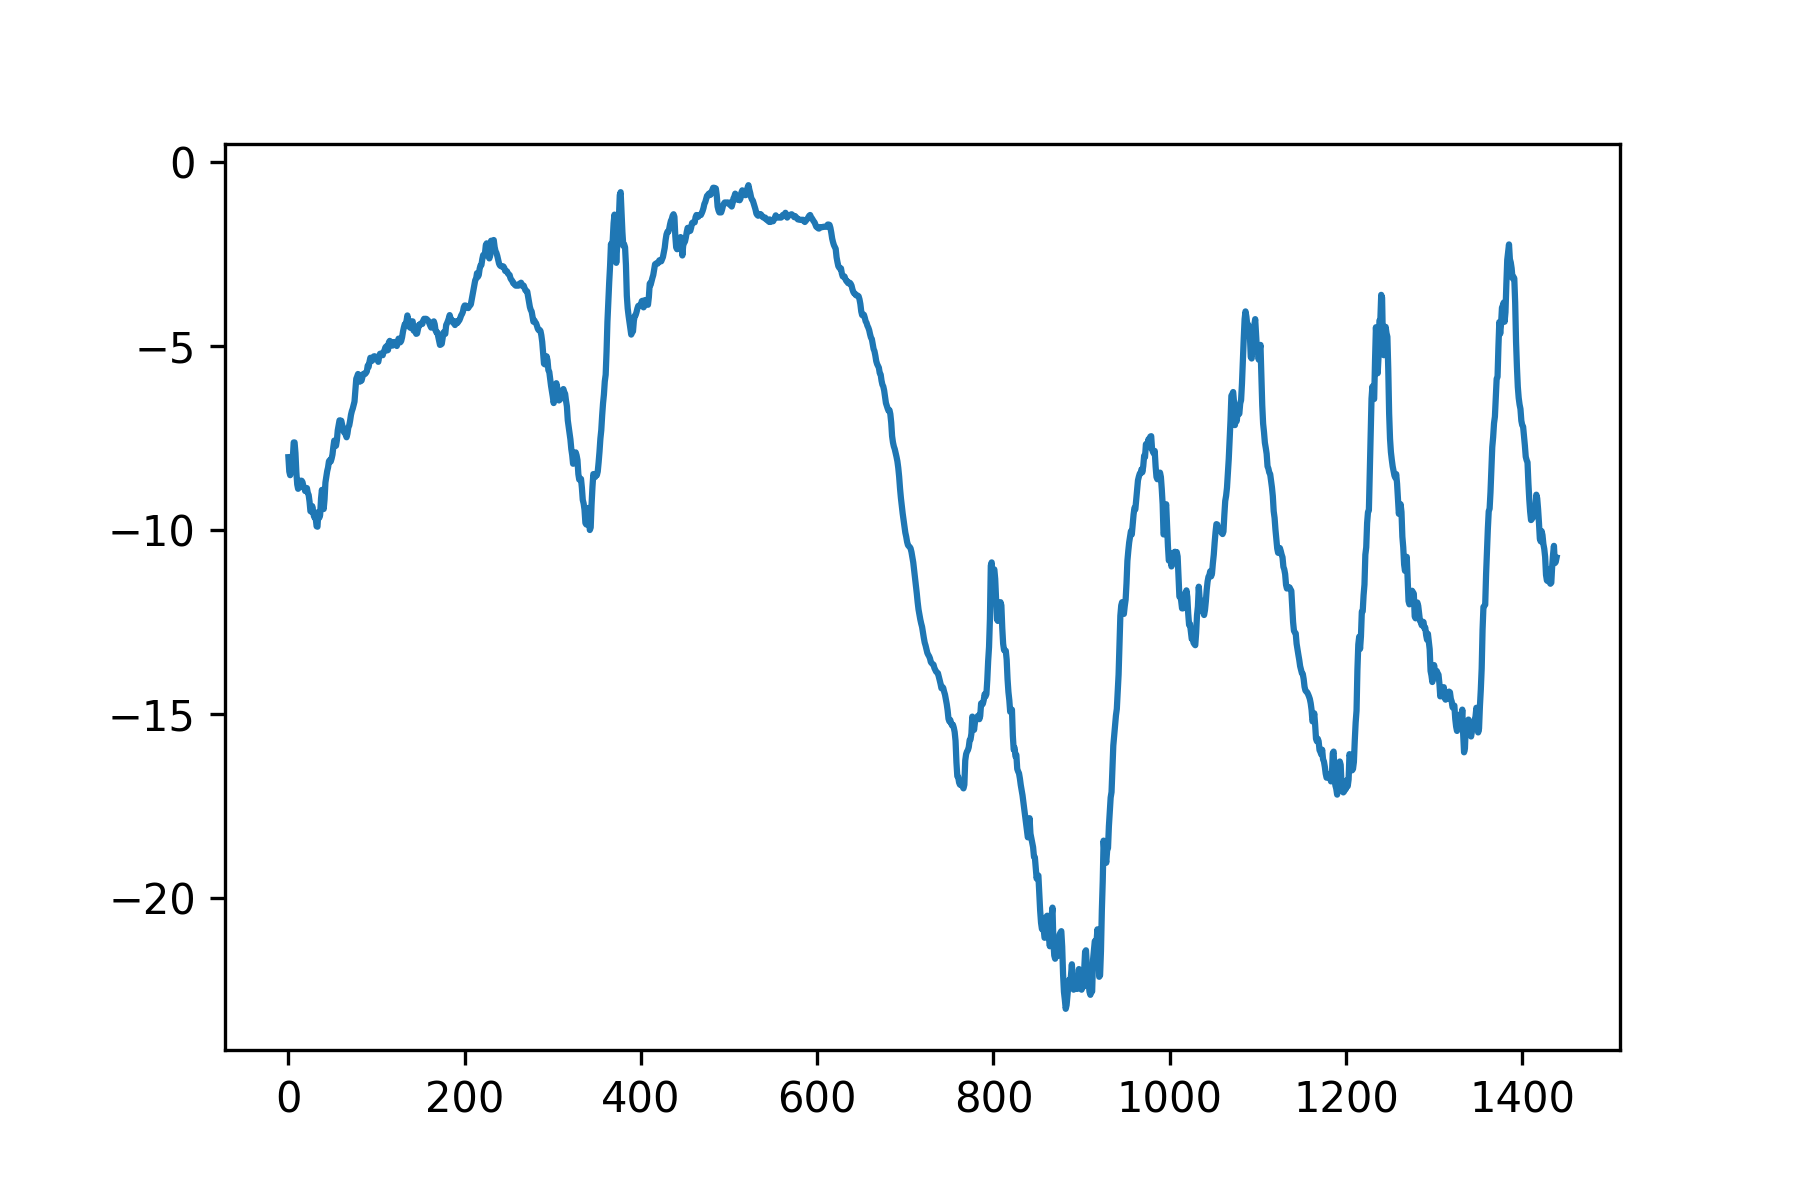
\includegraphics[width=\textwidth,height=0.6\textheight,keepaspectratio]{../../images/ch13/temperature_over_several_days.975eb51a.png}
            \caption{Nhiệt độ biến động trong vài ngày}
        \end{figure}
    \end{columns}
\end{frame}

\begin{frame}[fragile]{Tải và Đọc Dữ liệu Jena Weather}
Dữ liệu thời tiết Jena được lưu dưới định dạng \texttt{csv}. Chúng ta dùng Python để đọc dòng dữ liệu:
\begin{lstlisting}[language=Python]
import os

# Define the file path
fname = os.path.join("jena_climate_2009_2016.csv")

# Read the file
with open(fname) as f:
    data = f.read()

# Split by newlines
lines = data.split("\n")
header = lines[0].split(",")
lines = lines[1:]

print("Header features:", header)
print("Total timesteps:", len(lines)) # 420,551 lines
\end{lstlisting}
\end{frame}

\begin{frame}[fragile]{Chuyển đổi dữ liệu sang Numpy Array}
Chuyển đổi file CSV thành 2 mảng Numpy: mảng \texttt{temperature} dùng làm Target (mục tiêu dự báo) và \texttt{raw\_data} làm Input Features.
\begin{lstlisting}[language=Python]
import numpy as np

# Arrays for features and targets
temperature = np.zeros((len(lines),))
raw_data = np.zeros((len(lines), len(header) - 1))

for i, line in enumerate(lines):
    # Skip the Date Time column (index 0)
    values = [float(x) for x in line.split(",")[1:]]
    
    # Column 1 is temperature (T (degC))
    temperature[i] = values[1]
    
    # Store all columns in raw_data (including temperature)
    raw_data[i, :] = values[:]
\end{lstlisting}
\end{frame}

\begin{frame}[fragile]{Phân chia tập dữ liệu (Train/Val/Test)}
Khi làm việc với chuỗi thời gian, ta \textbf{không được xáo trộn ngẫu nhiên (shuffle)} các mẫu. Thay vào đó, tập kiểm tra phải đến \textbf{sau} tập huấn luyện trên trục thời gian.
\begin{lstlisting}[language=Python]
# First 50% for training
num_train_samples = int(0.5 * len(raw_data))

# Next 25% for validation
num_val_samples = int(0.25 * len(raw_data))

# Remaining 25% for testing
num_test_samples = len(raw_data) - num_train_samples - num_val_samples

print("num_train_samples:", num_train_samples)
print("num_val_samples:", num_val_samples)
print("num_test_samples:", num_test_samples)
\end{lstlisting}
\end{frame}

\begin{frame}[fragile]{Chuẩn hóa Dữ liệu (Normalization)}
Các đại lượng đo lường có đơn vị và biên độ khác nhau (áp suất khoảng $1000$ mbar, độ ẩm phần trăm từ $0-100$). Chuẩn hóa (Z-score) giúp mô hình hội tụ nhanh hơn.
\begin{lstlisting}[language=Python]
# Calculate mean and standard deviation ONLY on the training split
# to prevent data leakage from the future
mean = raw_data[:num_train_samples].mean(axis=0)
raw_data -= mean

std = raw_data[:num_train_samples].std(axis=0)
raw_data /= std
\end{lstlisting}
\begin{itemize}
    \item \textbf{Lưu ý quan trọng}: Tuyệt đối không tính \texttt{mean} hay \texttt{std} trên toàn bộ \texttt{raw\_data}. Nó vi phạm nguyên tắc "Mô hình không được biết thông tin của tương lai".
\end{itemize}
\end{frame}

\section{2. Xây dựng Dữ liệu và Các Baseline}

\begin{frame}[fragile]{Định nghĩa tham số Cửa sổ Thời gian (Time Window)}
Mục tiêu: Dùng dữ liệu 5 ngày liên tục (120 giờ) để dự báo thời tiết của 24 giờ kế tiếp.
\begin{lstlisting}[language=Python]
# Observations are sampled every 10 minutes (6 times an hour)
sampling_rate = 6

# We use the past 5 days (120 hours) as our input sequence
sequence_length = 120

# We want to predict the temperature 24 hours into the future
delay = sampling_rate * (sequence_length + 24 - 1)

# Batch size for neural networks
batch_size = 256
\end{lstlisting}
\end{frame}

\begin{frame}[fragile]{Khởi tạo Timeseries Generator của Keras}
Hàm \texttt{timeseries\_dataset\_from\_array} giúp tạo tự động các chuỗi nối tiếp từ dữ liệu thô mà không tốn quá nhiều RAM.
\begin{lstlisting}[language=Python]
import keras

train_dataset = keras.utils.timeseries_dataset_from_array(
    raw_data[:-delay],
    targets=temperature[delay:],
    sampling_rate=sampling_rate,
    sequence_length=sequence_length,
    shuffle=True, # Shuffle BATCHES, not the timeline itself
    batch_size=batch_size,
    start_index=0,
    end_index=num_train_samples,
)
\end{lstlisting}
Tương tự, ta tạo \texttt{val\_dataset} và \texttt{test\_dataset} bằng cách thay đổi \texttt{start\_index} và \texttt{end\_index}.
\end{frame}

\begin{frame}[fragile]{Một Baseline Suy luận Thông thường (Commonsense Baseline)}
Trực giác con người: Thời tiết ngày mai sẽ khá giống thời tiết ngày hôm nay. Vậy nếu dự báo "Nhiệt độ 24h tới = Nhiệt độ hiện tại" thì sai số là bao nhiêu?
\begin{lstlisting}[language=Python]
def evaluate_naive_method(dataset):
    total_abs_err = 0.0
    samples_seen = 0
    for samples, targets in dataset:
        # Predict the last temperature in the sequence
        # Temperature is column 1 (index 1)
        preds = samples[:, -1, 1] * std[1] + mean[1]
        
        # Calculate Absolute Error
        total_abs_err += np.sum(np.abs(preds - targets))
        samples_seen += samples.shape[0]
    return total_abs_err / samples_seen

print(f"Validation MAE: {evaluate_naive_method(val_dataset):.2f}")
\end{lstlisting}
Sai số trung bình tuyệt đối (MAE) của phương pháp ngây ngô này là \textbf{2.44 độ C}. Bất kì AI nào muốn hoạt động hiệu quả cũng phải có Loss thấp hơn con số này.
\end{frame}

\begin{frame}[fragile]{Sự thất bại của mạng Densely-connected Model}
Thử nghiệm Feed-forward Network truyền thống. Chúng ta trải phẳng (Flatten) mảng thời gian thành Vector 1D.
\begin{lstlisting}[language=Python]
from keras import layers

inputs = keras.Input(shape=(sequence_length, raw_data.shape[-1]))
# Flatten the sequence: destroys the concept of "time"
x = layers.Flatten()(inputs)
x = layers.Dense(16, activation="relu")(x)
outputs = layers.Dense(1)(x) # Output is continuous prediction

model = keras.Model(inputs, outputs)
model.compile(optimizer="adam", loss="mse", metrics=["mae"])

history = model.fit(train_dataset, epochs=10, 
                    validation_data=val_dataset)
\end{lstlisting}
\end{frame}

\begin{frame}{Biểu đồ Loss của Densely-connected Model}
    \begin{columns}
        \column{0.5\textwidth}
        \begin{itemize}
            \item Trải phẳng (Flatten) chuỗi thời gian và đưa qua các lớp \texttt{Dense}.
            \item \textbf{Kết quả:} Loss trên tập Validation (Đường liền) bị bão hòa nhanh chóng, Overfit. Validation MAE khoảng $2.6$ độ C, tệ hơn cả Baseline ($2.44$).
            \item \textbf{Nguyên nhân:} Mạng Dense loại bỏ hoàn toàn khái niệm "Thời gian". Nó xem mọi điểm dữ liệu trong chuỗi là độc lập (IID).
        \end{itemize}
        
        \column{0.5\textwidth}
        \begin{figure}
            \centering
            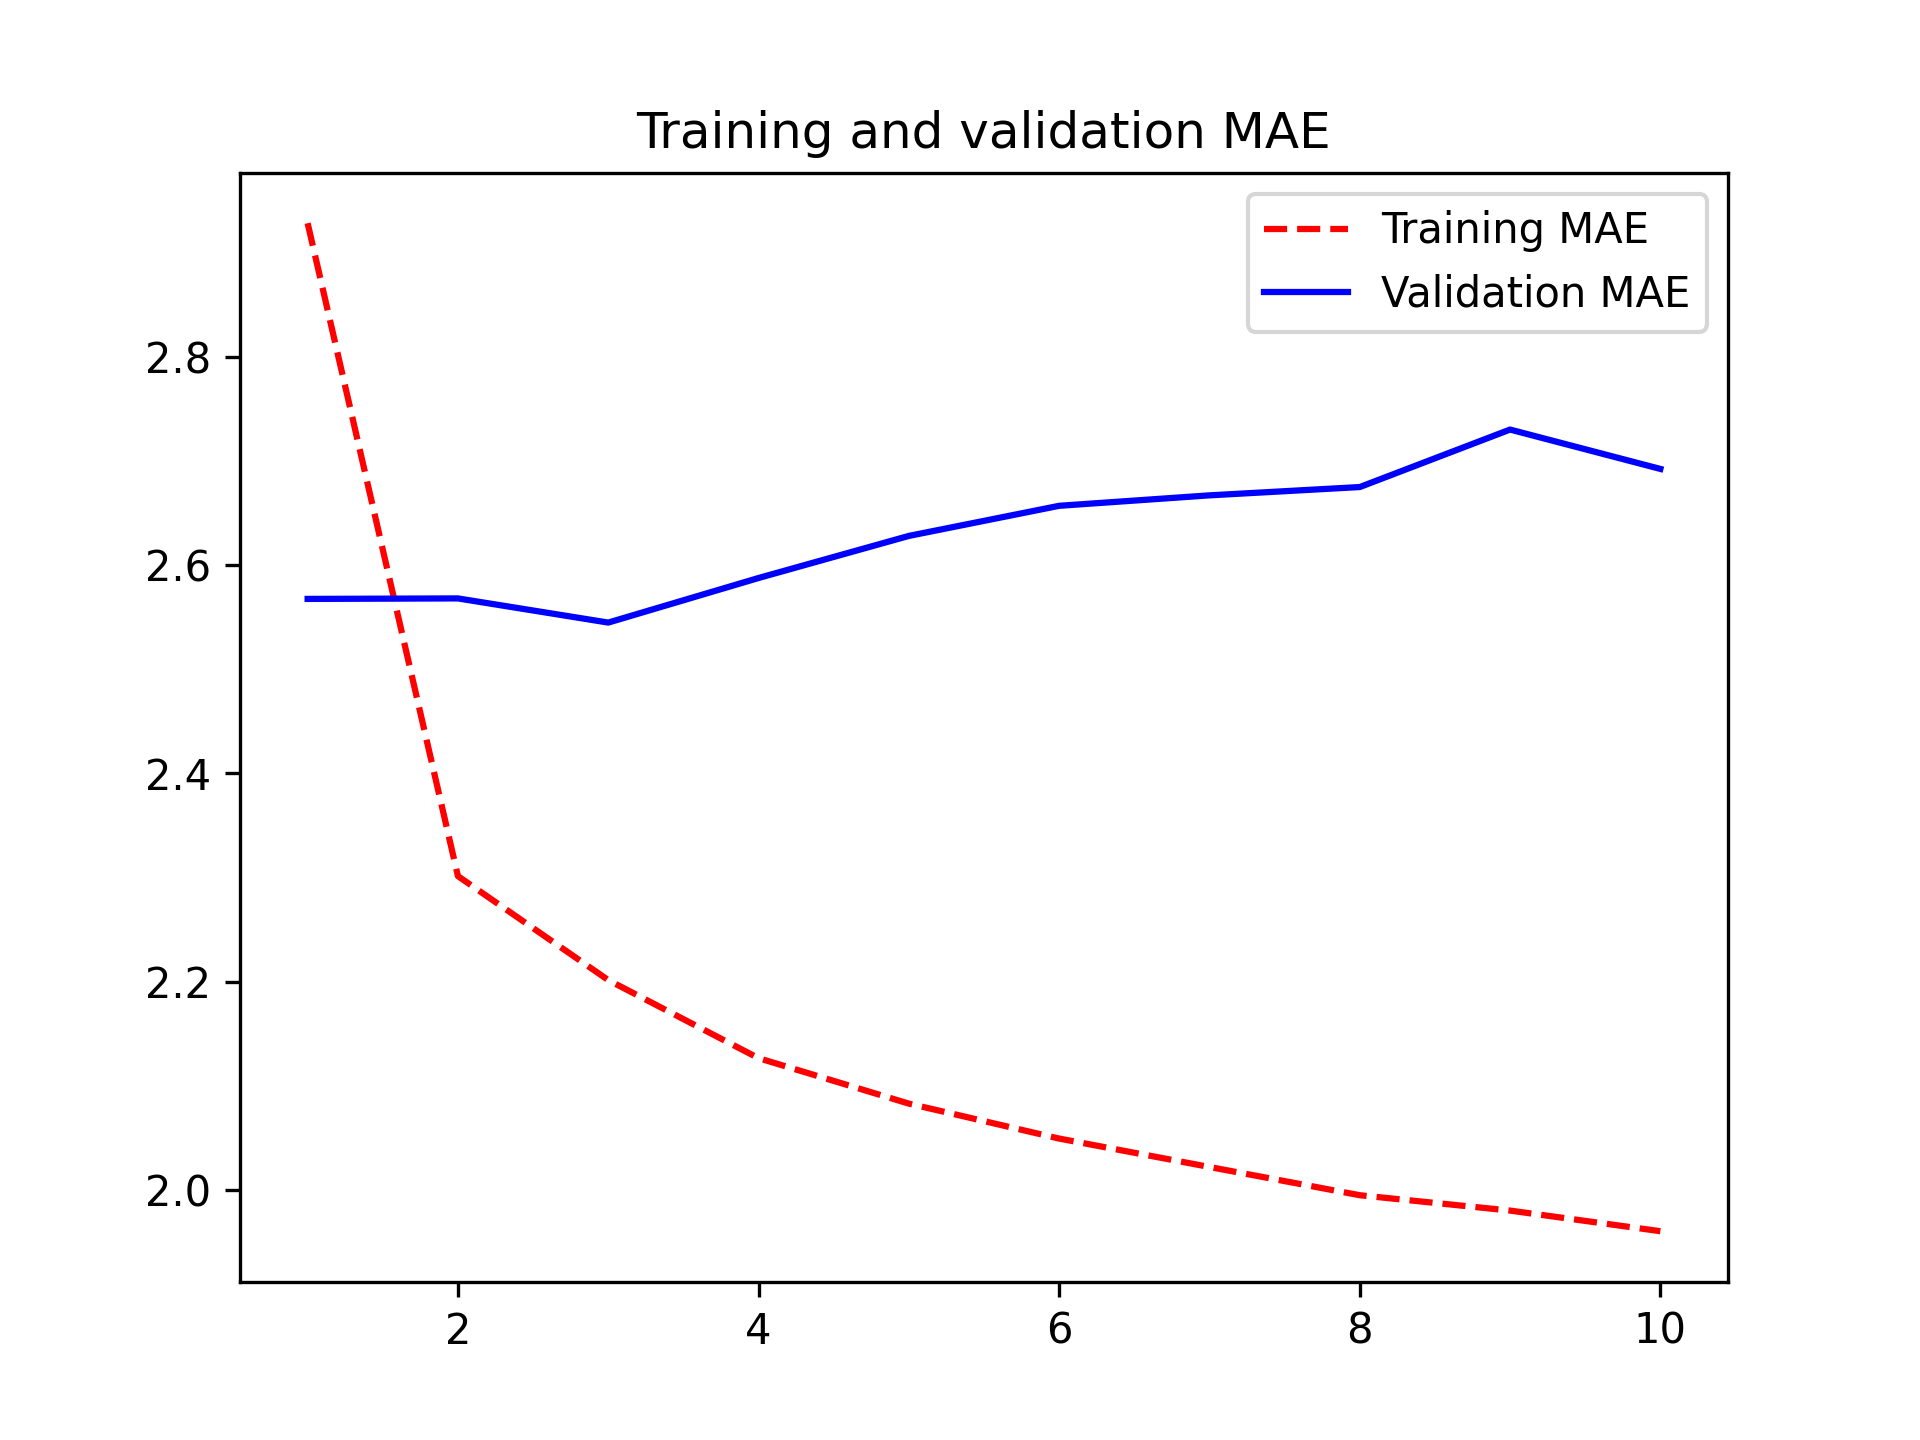
\includegraphics[width=\textwidth,height=0.6\textheight,keepaspectratio]{../../images/ch13/dense_model_metrics.8448f47a.png}
            \caption{Training Loss của Dense Model}
        \end{figure}
    \end{columns}
\end{frame}

\begin{frame}[fragile]{Thử nghiệm với Mạng 1D Convolution}
Thay đổi kiến trúc bằng mạng Tích chập 1 chiều (1D ConvNet) với hi vọng trích xuất đặc trưng lặp lại cục bộ.
\begin{lstlisting}[language=Python]
inputs = keras.Input(shape=(sequence_length, raw_data.shape[-1]))
# Swipe a 1D window across sequence
x = layers.Conv1D(8, 24, activation="relu")(inputs)
x = layers.MaxPooling1D(2)(x)
x = layers.Conv1D(8, 12, activation="relu")(x)
x = layers.MaxPooling1D(2)(x)
x = layers.Conv1D(8, 6, activation="relu")(x)
x = layers.GlobalAveragePooling1D()(x) # Collapse time dimension

outputs = layers.Dense(1)(x)
model = keras.Model(inputs, outputs)
model.compile(optimizer="adam", loss="mse", metrics=["mae"])
\end{lstlisting}
\end{frame}

\begin{frame}{Biểu đồ Loss của Mạng 1D Convolution}
    \begin{columns}
        \column{0.5\textwidth}
        \begin{itemize}
            \item \textbf{Kết quả:} Validation MAE rơi vào khoảng $2.9$ độ C. Tệ hơn cả Mạng Dense!
            \item \textbf{Lý do:} Conv1D giả định ranh giới Dịch chuyển Bất biến (Translation Invariance). Nghĩa là một khuôn mẫu ở thứ 2 có ý nghĩa giống hệt thứ 5. 
            \item Điều này sai lầm trong Timeseries vì thời gian \textbf{càng gần hiện tại càng mang thông tin quan trọng}. Tính chất Max Pooling cũng vô tình xóa sạch khái niệm thứ tự (Order).
        \end{itemize}
        
        \column{0.5\textwidth}
        \begin{figure}
            \centering
            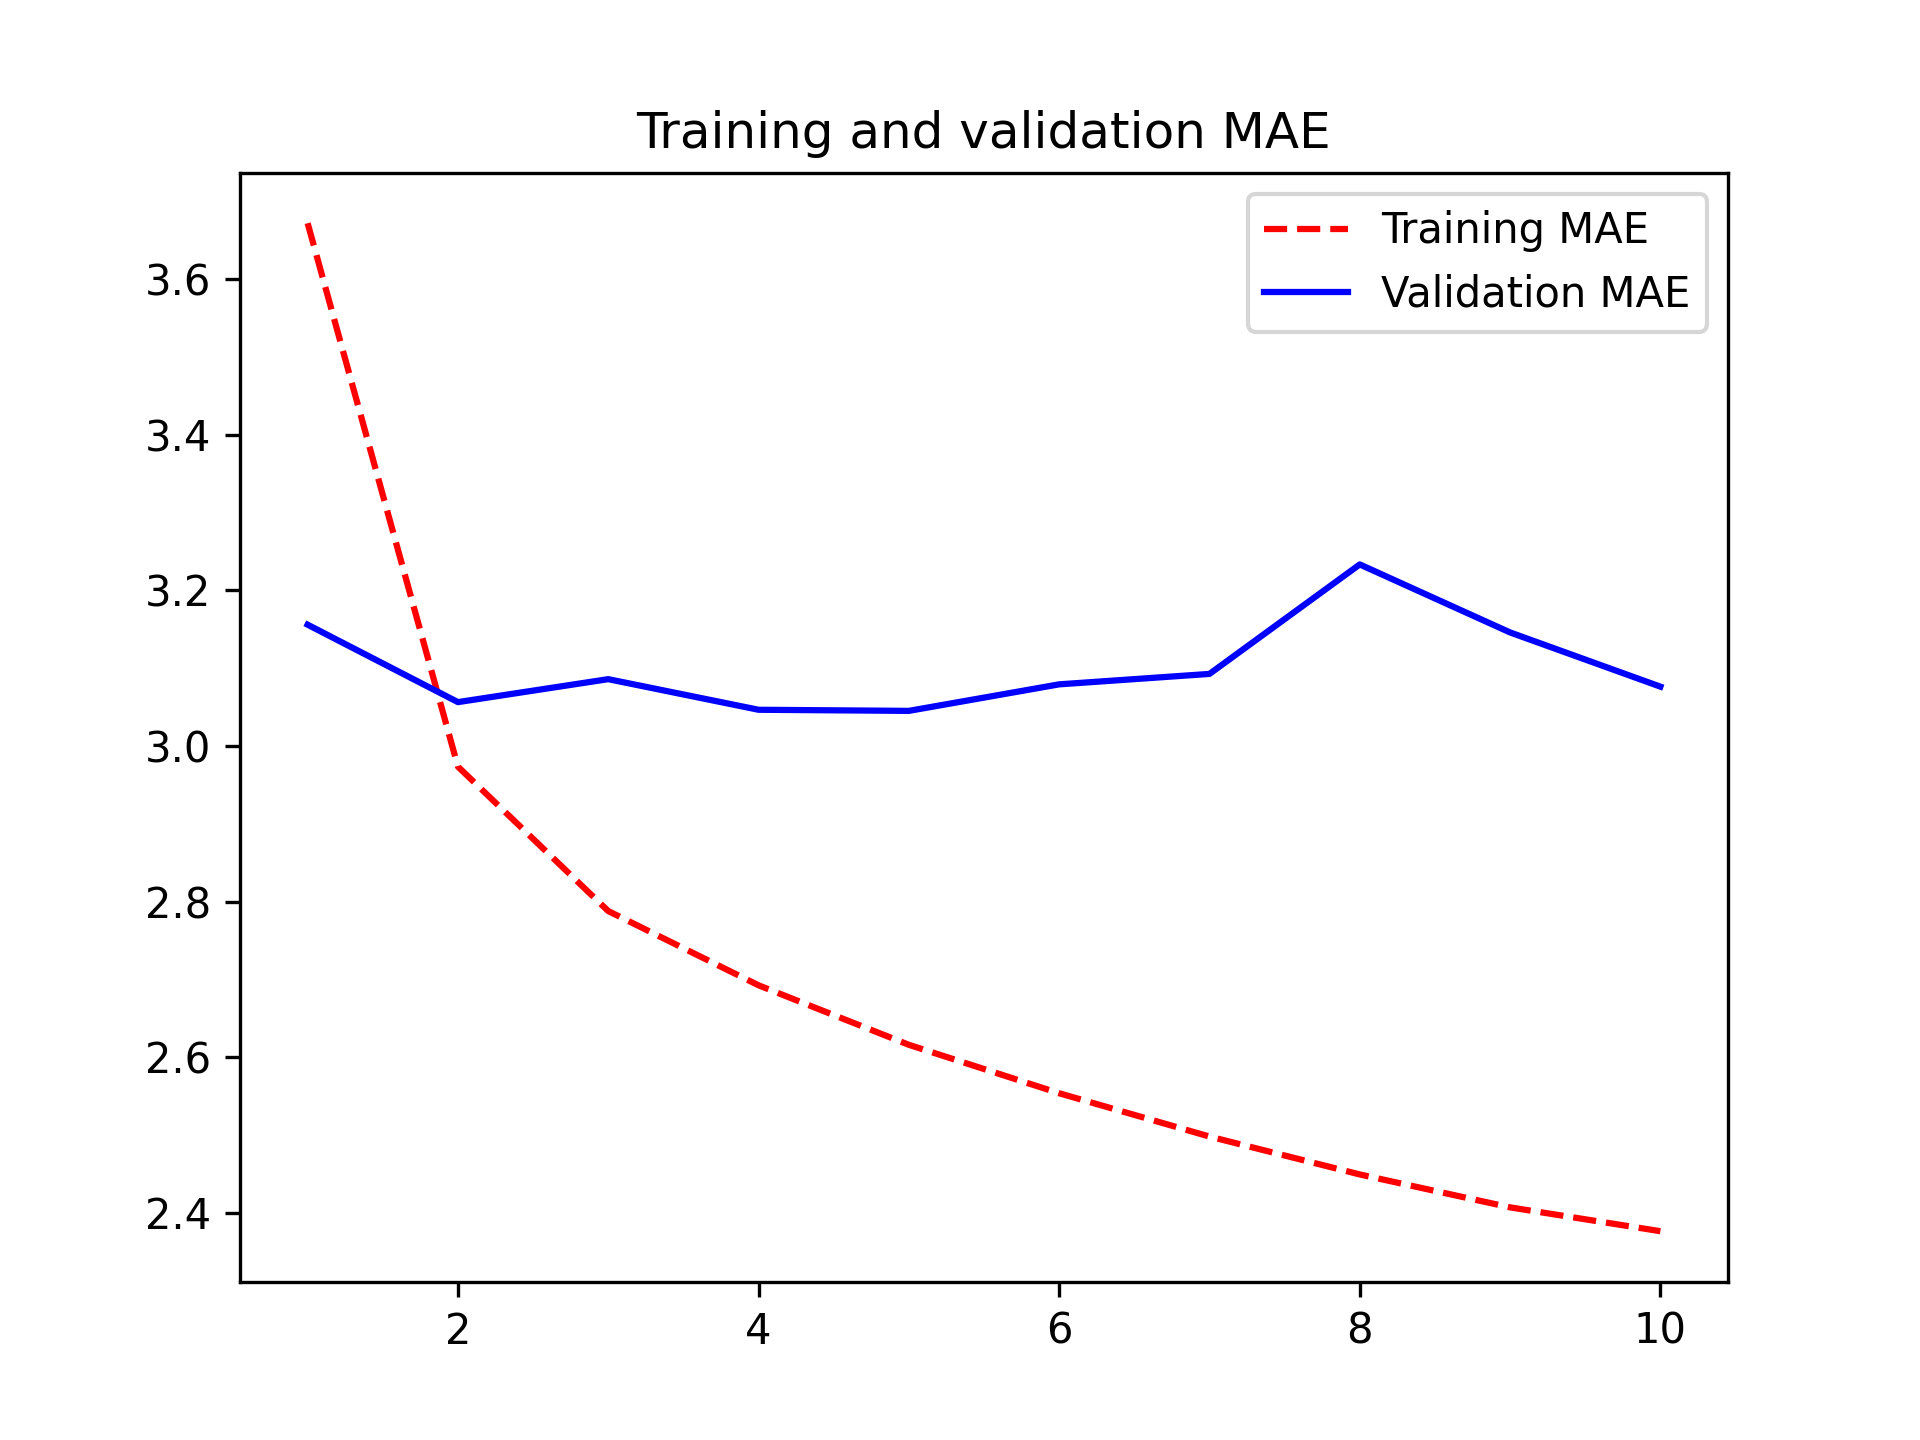
\includegraphics[width=\textwidth,height=0.6\textheight,keepaspectratio]{../../images/ch13/conv_model_metrics.fe487977.png}
            \caption{Training Loss của 1D Conv}
        \end{figure}
    \end{columns}
\end{frame}

\section{3. Mạng Nơ-ron Truyền hồi (Recurrent Neural Networks - RNN)}

\begin{frame}{Khái niệm Mạng Nơ-ron Truyền hồi (RNN)}
    \begin{columns}
        \column{0.5\textwidth}
        \begin{itemize}
            \item Trái ngược với mạng Feed-forward, RNN duy trì một \textbf{Trạng thái (State)} đóng vai trò như "Bộ nhớ".
            \item Nó duyệt qua từng bước thời gian $t$, tính toán Đầu ra (Output) tại $t$, và cập nhật lại Trạng thái để dùng cho $t+1$.
            \item RNN lưu giữ thông tin về những gì nó đã thấy cho đến nay.
        \end{itemize}
        
        \column{0.5\textwidth}
        \begin{figure}
            \centering
            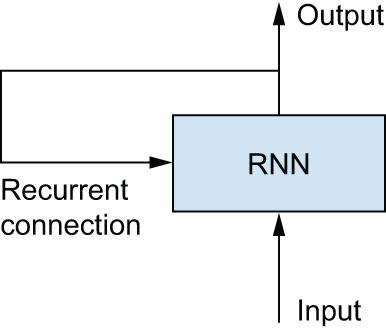
\includegraphics[width=\textwidth,height=0.6\textheight,keepaspectratio]{../../images/ch13/simplernn.822d53ed.png}
            \caption{Vòng lặp trong mạng SimpleRNN}
        \end{figure}
    \end{columns}
\end{frame}

\begin{frame}[fragile]{Vòng lặp bên trong mô hình RNN (Giả lập)}
Khác với vòng lặp \texttt{for} bình thường, trạng thái của một vòng lặp RNN được lưu vết lại để tính cho bước tiếp theo.
\begin{lstlisting}[language=Python]
state_t = 0 # The state at time t
for input_t in input_sequence:
    # Function f combines input and current state using weights
    # output_t = activation(dot(W, input_t) + dot(U, state_t) + b)
    output_t = f(input_t, state_t)
    
    # The previous output becomes the state for the next iteration.
    state_t = output_t
\end{lstlisting}
Trạng thái này được khởi tạo bằng $0$ lúc bắt đầu một chuỗi.
\end{frame}

\begin{frame}[fragile]{Lớp SimpleRNN trong Keras}
Mặc định RNN chỉ trả về Trạng thái Ẩn cuối cùng (Last State Output) mang theo toàn bộ ký ức. Nếu muốn giữ nguyên các trạng thái trung gian, cấu hình \texttt{return\_sequences}.
\begin{lstlisting}[language=Python]
num_features = 14
inputs = keras.Input(shape=(None, num_features))

# 1. Return ONLY the final output (Shape: (None, 16))
outputs = layers.SimpleRNN(16, return_sequences=False)(inputs)

# 2. Return the FULL sequence (Shape: (None, timesteps, 16))
outputs = layers.SimpleRNN(16, return_sequences=True)(inputs)

# Stacking RNNs requires return_sequences=True
x = layers.SimpleRNN(16, return_sequences=True)(inputs)
x = layers.SimpleRNN(16, return_sequences=True)(x)
outputs = layers.SimpleRNN(16)(x)
\end{lstlisting}
\end{frame}

\begin{frame}{Vấn đề cốt lõi: Vanishing Gradients (Triệt tiêu Đạo hàm)}
    \begin{itemize}
        \item Mạng \textbf{SimpleRNN} hoạt động tốt về mặt lý thuyết, nhưng thất bại trong thực tế.
        \item Khi độ dài chuỗi tăng lên, Đạo hàm (Gradient) từ tương lai phải nhân liên tục qua hàng trăm ma trận trọng số để quay ngược về quá khứ.
        \item Nếu các ma trận trọng số nhỏ hơn $1$, đạo hàm sẽ tiến về $0$ cực nhanh (Triệt tiêu).
        \item Hậu quả: SimpleRNN bị "mất trí nhớ" ngắn hạn, quên mất các thông tin đầu chuỗi. Mạng dừng học.
    \end{itemize}
\end{frame}

\section{4. Kiến trúc LSTM - Long Short-Term Memory}

\begin{frame}{Giải pháp LSTM: Bổ sung Trạng thái Tế bào (Cell State)}
    \begin{itemize}
        \item Được phát minh năm 1997, LSTM bổ sung một đường chuyền dữ liệu song song gọi là \textbf{Cell State ($C_t$)}.
        \item Tưởng tượng $C_t$ như một băng chuyền chạy dọc qua toàn bộ chuỗi. Thông tin có thể dễ dàng chảy xuyên suốt mà không bị thay đổi quá nhiều (Giải quyết hoàn toàn Vanishing Gradients).
        \item Các \textbf{Cổng (Gates)} sẽ quyết định thêm/bớt thông tin gì vào dải băng chuyền này.
    \end{itemize}
\end{frame}

\begin{frame}{LSTM (Phần 1): Trạng thái mang theo}
    \begin{columns}
        \column{0.5\textwidth}
        \begin{itemize}
            \item Tại thời điểm $t$, ta có Đầu vào $X_t$ và Trạng thái ẩn từ quá khứ $H_{t-1}$.
            \item Thay vì chỉ đưa ra $H_t$ như RNN thông thường, LSTM truyền thêm $C_{t-1}$ vào ô tế bào hiện tại.
        \end{itemize}
        
        \column{0.5\textwidth}
        \begin{figure}
            \centering
            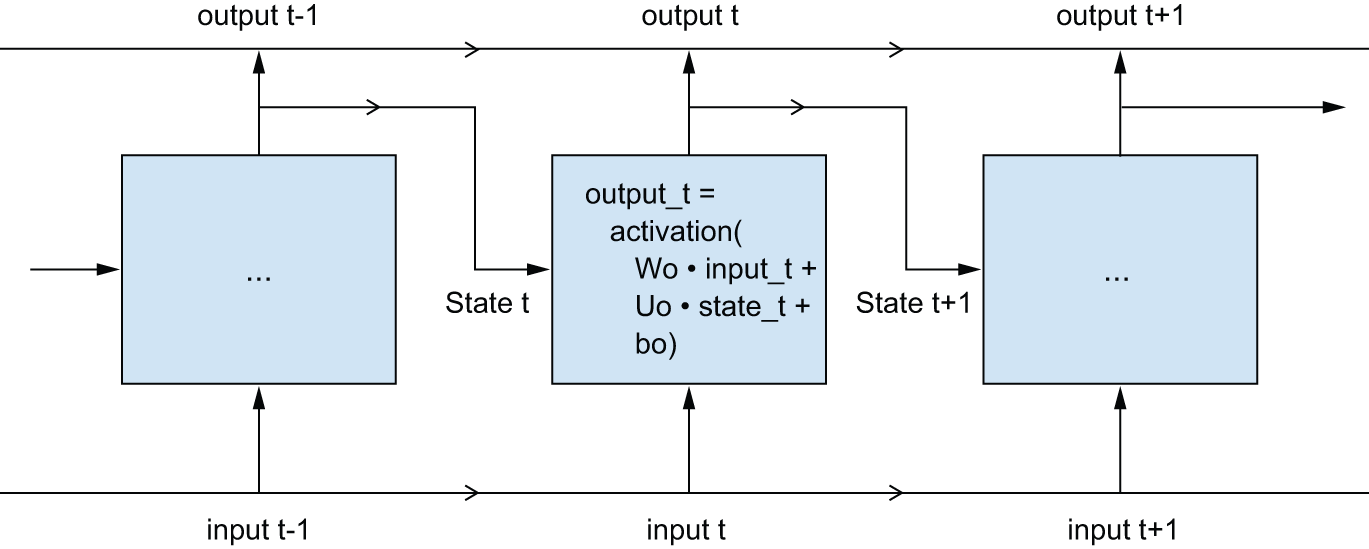
\includegraphics[width=\textwidth,height=0.6\textheight,keepaspectratio]{../../images/ch13/unrolled_lstm_1.d9bee30c.png}
            \caption{Giai đoạn khởi nhập của LSTM}
        \end{figure}
    \end{columns}
\end{frame}

\begin{frame}{LSTM (Phần 2): Forget Gate và Input Gate}
    \begin{columns}
        \column{0.5\textwidth}
        Tính toán Tế bào trạng thái mới $C_t$:
        \begin{enumerate}
            \item \textbf{Forget Gate ($f$):} Quên bớt thông tin cũ không còn quan trọng. Hàm Sigmoid xuất giá trị $0$ (Xóa) đến $1$ (Giữ lại).
            $$ f = \sigma(W_f \cdot [X_t, H_{t-1}] + b_f) $$
            \item \textbf{Input Gate ($i$ và $k$):} Tạo thông tin mới để cập nhật vào băng chuyền.
            $$ i = \sigma(W_i \cdot [X_t, H_{t-1}] + b_i) $$
            $$ k = \tanh(W_k \cdot [X_t, H_{t-1}] + b_k) $$
            \item $C_t = C_{t-1} * f + i * k$
        \end{enumerate}
        
        \column{0.5\textwidth}
        \begin{figure}
            \centering
            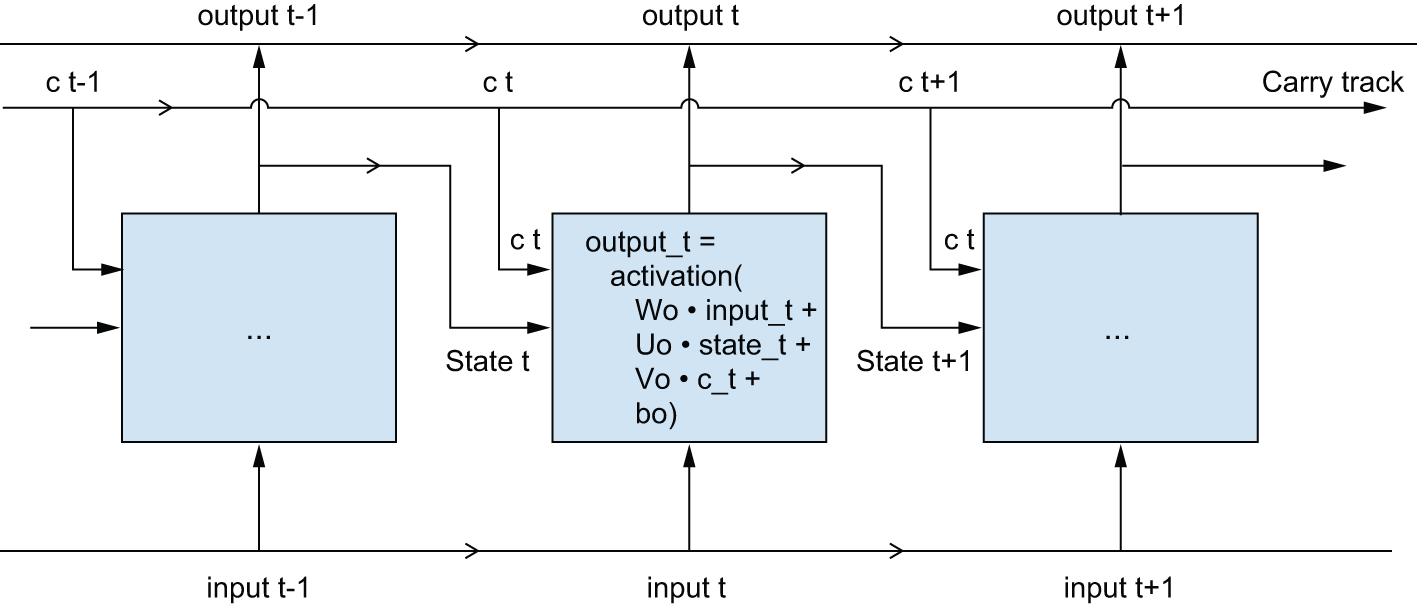
\includegraphics[width=\textwidth,height=0.6\textheight,keepaspectratio]{../../images/ch13/unrolled_lstm_2.4145ecdf.png}
            \caption{Cập nhật Cell State $c_t$}
        \end{figure}
    \end{columns}
\end{frame}

\begin{frame}{LSTM (Phần 3): Output Gate}
    \begin{columns}
        \column{0.5\textwidth}
        Cuối cùng, tính Trạng thái ẩn $H_t$ (Cũng chính là Output):
        \begin{itemize}
            \item \textbf{Output Gate ($o$):} Quyết định phần nào của Cell State sẽ được xuất ra.
            $$ o = \sigma(W_o \cdot [X_t, H_{t-1}] + b_o) $$
            \item Tính toán $H_t$:
            $$ H_t = o * \tanh(C_t) $$
            \item Trạng thái ẩn $H_t$ mang thông tin tinh lọc nhất để chuẩn bị bước sang thời điểm $t+1$.
        \end{itemize}
        
        \column{0.5\textwidth}
        \begin{figure}
            \centering
            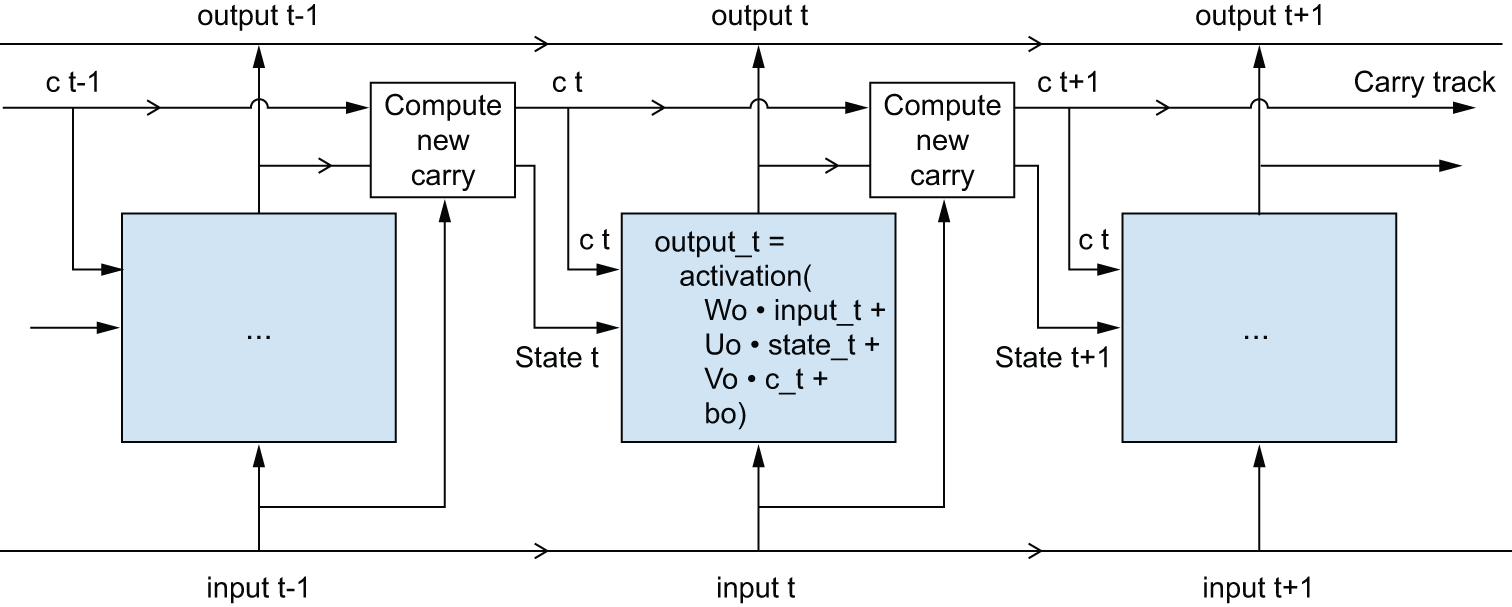
\includegraphics[width=\textwidth,height=0.6\textheight,keepaspectratio]{../../images/ch13/unrolled_lstm_3.1f68b33f.png}
            \caption{Xuất giá trị $h_t$}
        \end{figure}
    \end{columns}
\end{frame}

\begin{frame}[fragile]{Xây dựng mô hình LSTM với Keras}
Mặc dù thuật toán phức tạp, nhưng việc triển khai lại cực kỳ đơn giản với Keras qua class \texttt{LSTM}.
\begin{lstlisting}[language=Python]
inputs = keras.Input(shape=(sequence_length, raw_data.shape[-1]))

# The LSTM layer handles all the internal memory cell logic
x = layers.LSTM(16)(inputs)
outputs = layers.Dense(1)(x)

model = keras.Model(inputs, outputs)
model.compile(optimizer="adam", loss="mse", metrics=["mae"])

history = model.fit(train_dataset, epochs=10, 
                    validation_data=val_dataset)
\end{lstlisting}
\end{frame}

\begin{frame}{Hiệu suất Đột phá của LSTM}
    \begin{columns}
        \column{0.5\textwidth}
        \begin{itemize}
            \item \textbf{Kết quả:} Validation MAE giảm còn $2.39$ độ C, chính thức \textbf{vượt qua độ chính xác của Baseline} ($2.44$ độ C).
            \item Tuy nhiên, do số lượng tham số lớn, mô hình bắt đầu bị hiện tượng Overfit từ \texttt{Epoch 5} (Validation Loss cong dần lên).
            \item Cần các kỹ thuật nâng cao tiếp theo.
        \end{itemize}
        
        \column{0.5\textwidth}
        \begin{figure}
            \centering
            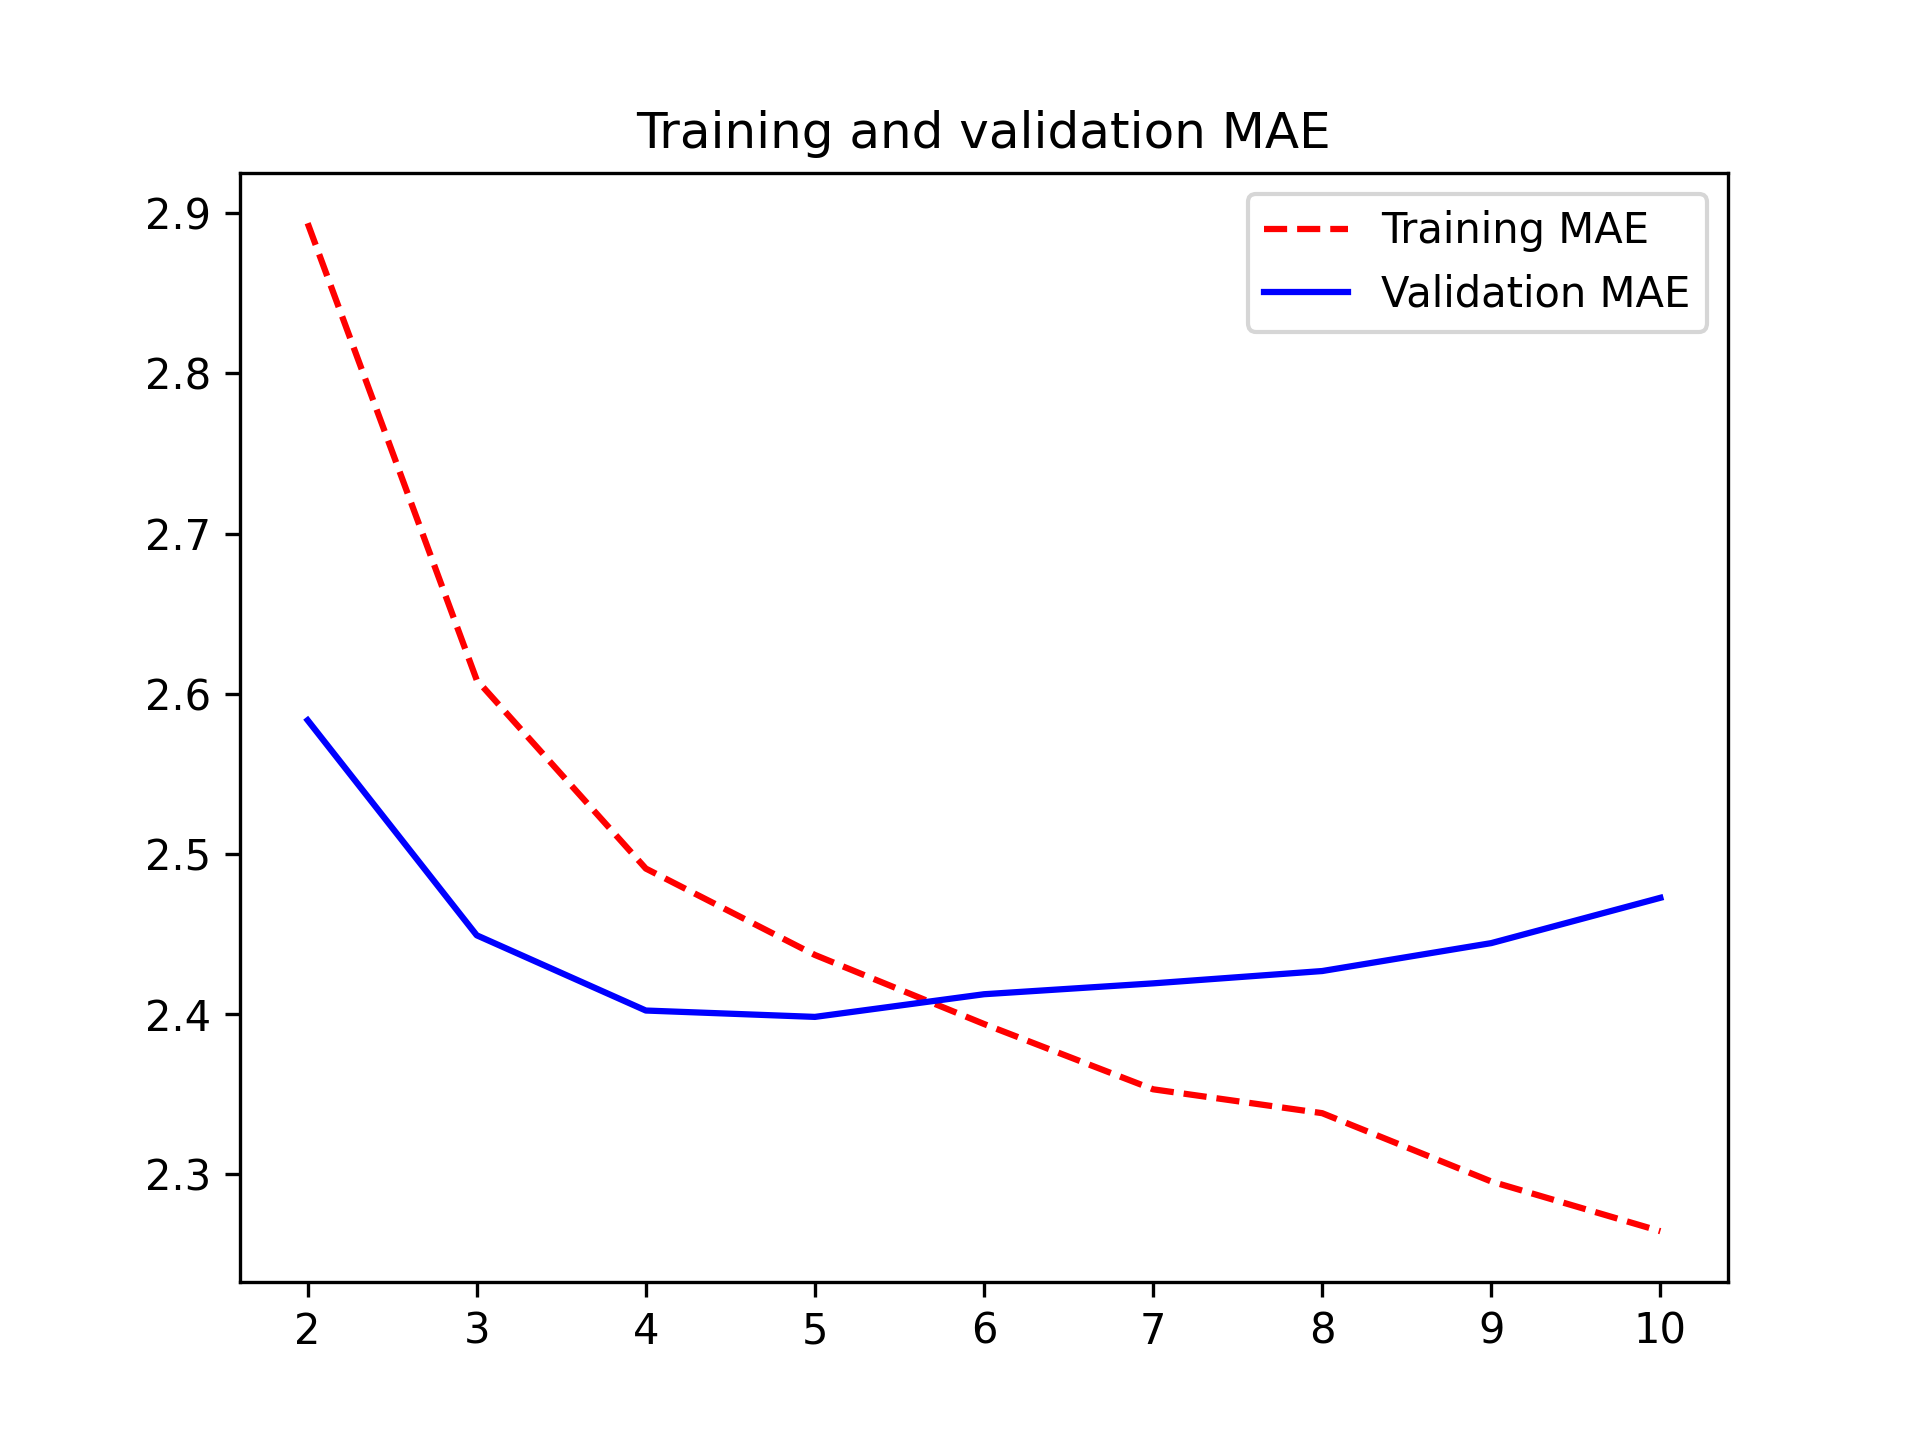
\includegraphics[width=\textwidth,height=0.6\textheight,keepaspectratio]{../../images/ch13/lstm_model_metrics.ae01dd09.png}
            \caption{Biểu đồ Loss của LSTM}
        \end{figure}
    \end{columns}
\end{frame}

\section{5. Các Kỹ thuật Nâng cao cho RNN}

\begin{frame}[fragile]{Kỹ thuật 1: Recurrent Dropout (Chống Overfitting)}
Dropout truyền thống có thể phá vỡ tính liên tục của thời gian. Keras cung cấp tham số \texttt{recurrent\_dropout} để tắt ngẫu nhiên nơ-ron "bên trong" tế bào LSTM thay vì chỉ tắt đầu vào.
\begin{lstlisting}[language=Python]
inputs = keras.Input(shape=(sequence_length, raw_data.shape[-1]))

# Apply recurrent_dropout to the hidden state connections
x = layers.LSTM(32, recurrent_dropout=0.25)(inputs)

# Standard dropout for the Dense head
x = layers.Dropout(0.5)(x)

outputs = layers.Dense(1)(x)
model = keras.Model(inputs, outputs)
model.compile(optimizer="adam", loss="mse", metrics=["mae"])
\end{lstlisting}
\end{frame}

\begin{frame}{Biểu đồ sức mạnh của Recurrent Dropout}
    \begin{columns}
        \column{0.5\textwidth}
        \begin{itemize}
            \item \textbf{Kết quả:} Mô hình duy trì độ ổn định tuyệt vời. Đường Validation và Training chạy sát nhau và không phân kì.
            \item Validation Loss giảm sâu hơn nữa xuống $2.27$ độ C (Cải thiện 7\% so với Baseline ban đầu).
            \item Quá trình huấn luyện không còn bị Overfit sớm, có thể tăng \texttt{Epochs} thoải mái.
        \end{itemize}
        
        \column{0.5\textwidth}
        \begin{figure}
            \centering
            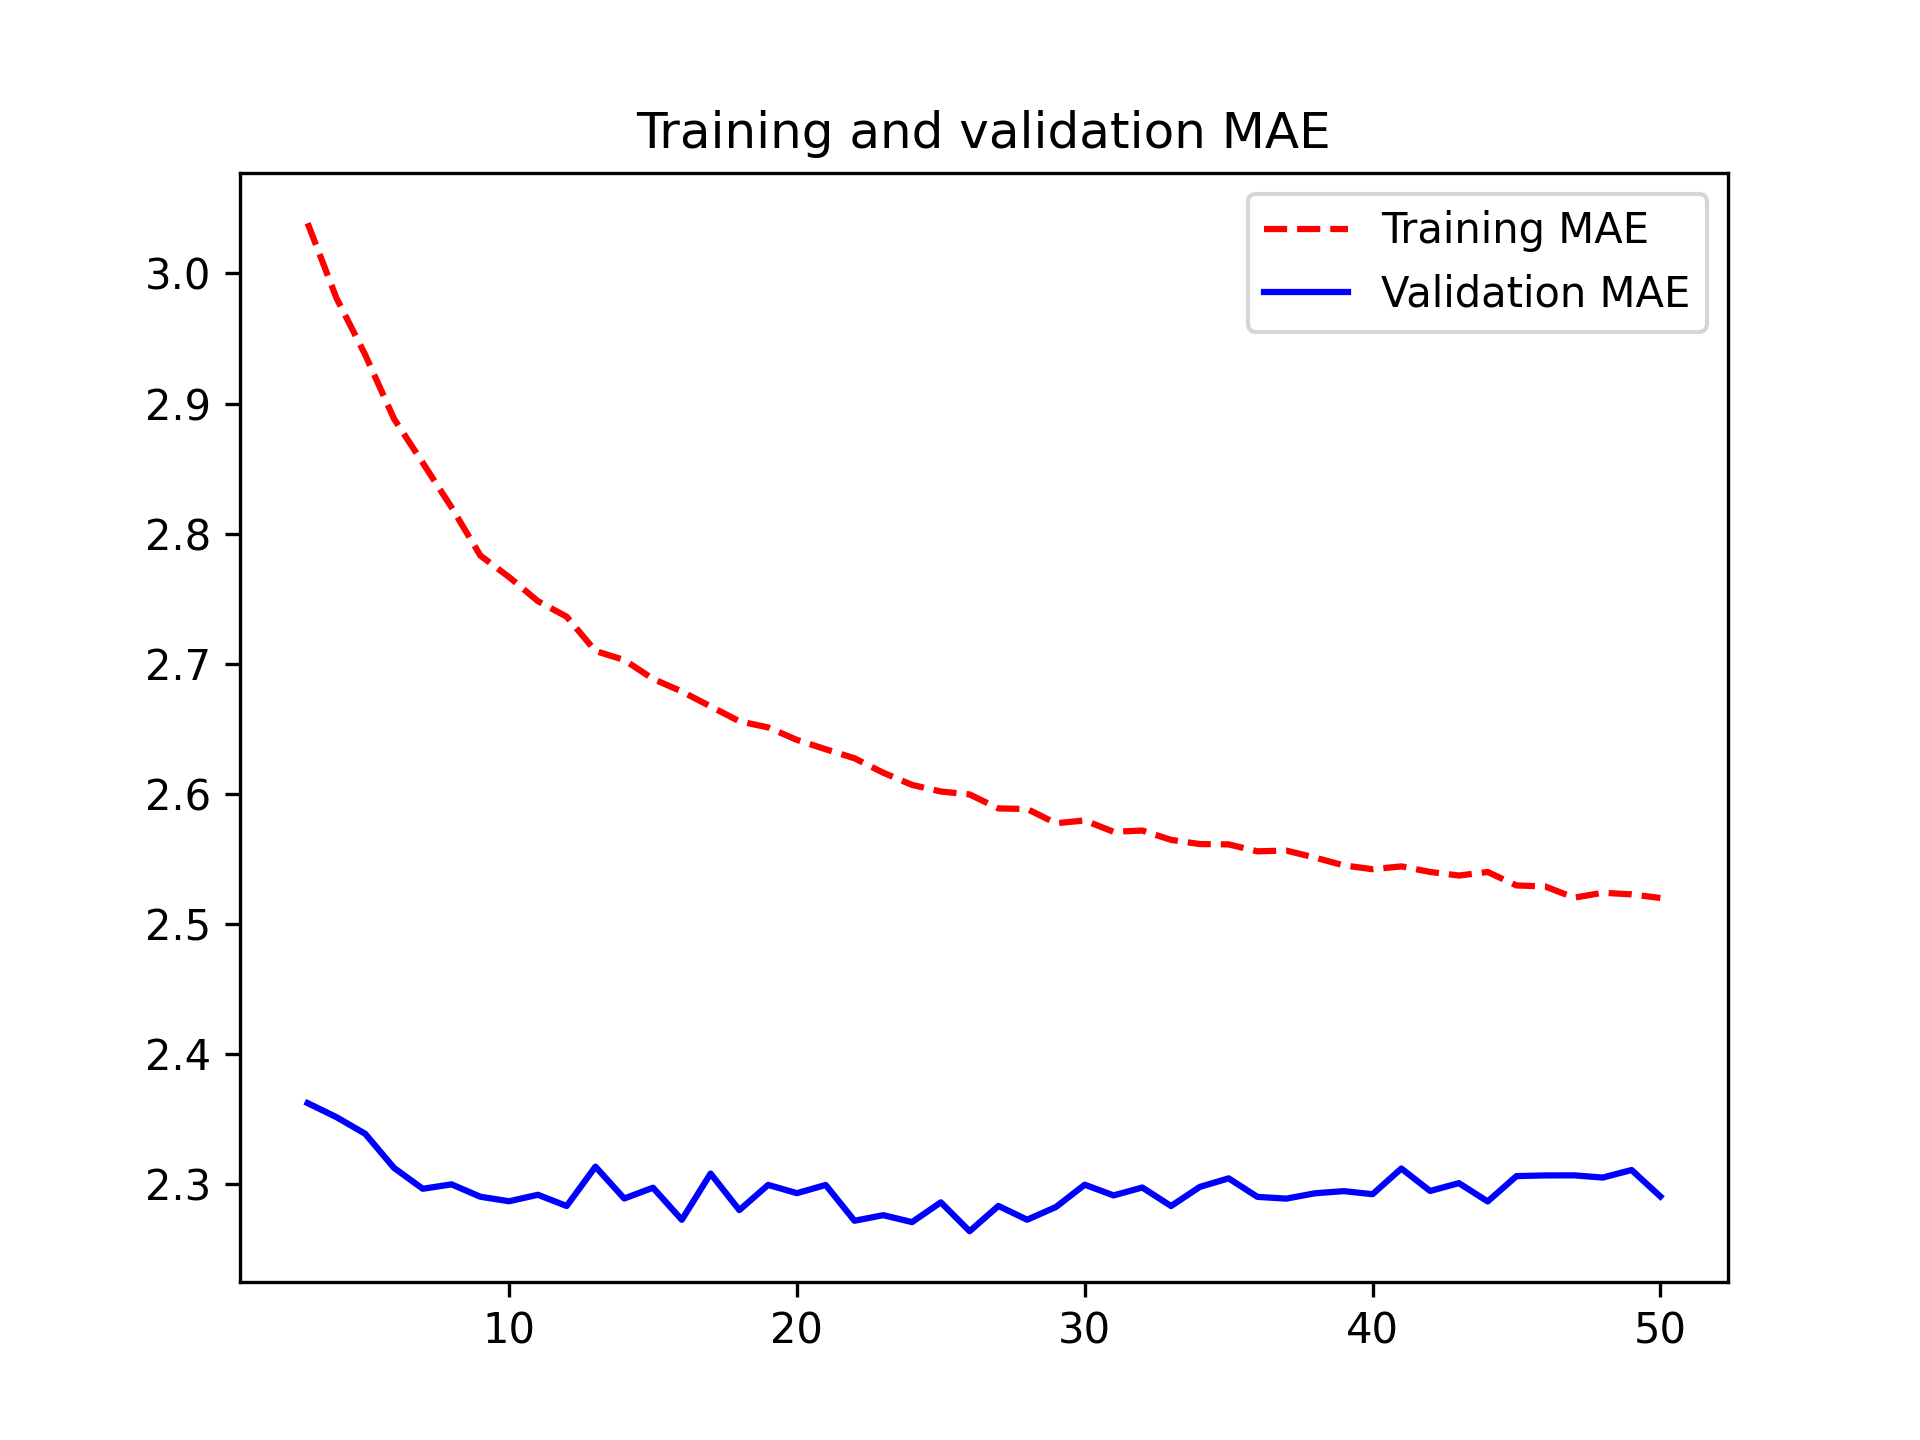
\includegraphics[width=\textwidth,height=0.6\textheight,keepaspectratio]{../../images/ch13/lstm_dropout_model_metrics.a624dc88.png}
            \caption{Sức mạnh của Recurrent Dropout}
        \end{figure}
    \end{columns}
\end{frame}

\begin{frame}[fragile]{Kỹ thuật 2: Xếp chồng RNN (Stacked GRU)}
Khi mô hình không còn Overfit, ta có thể an tâm tăng sức mạnh cấu trúc bằng cách Xếp chồng các lớp RNN. Sử dụng lớp \texttt{GRU} giúp tốc độ tính toán nhanh hơn.
\begin{lstlisting}[language=Python]
inputs = keras.Input(shape=(sequence_length, raw_data.shape[-1]))

# Bottom layer MUST return sequence for the next layer
x = layers.GRU(32, recurrent_dropout=0.5, return_sequences=True)(inputs)

# Top layer
x = layers.GRU(32, recurrent_dropout=0.5)(x)
x = layers.Dropout(0.5)(x)

outputs = layers.Dense(1)(x)
model = keras.Model(inputs, outputs)
\end{lstlisting}
\end{frame}

\begin{frame}{Biểu đồ Xếp chồng GRU + Dropout}
    \begin{columns}
        \column{0.5\textwidth}
        \begin{itemize}
            \item \textbf{Kết quả:} Mô hình tiếp tục hội tụ và cho kết quả ổn định. 
            \item Tăng dung lượng mạng đôi khi gặp phải "Lợi tức giảm dần" (Diminishing Returns), tức là mạng lớn hơn nhưng hiệu suất tăng không đáng kể. 
            \item GRU (Gated Recurrent Unit) là phiên bản tinh giản của LSTM nhưng đem lại hiệu quả tương đương.
        \end{itemize}
        
        \column{0.5\textwidth}
        \begin{figure}
            \centering
            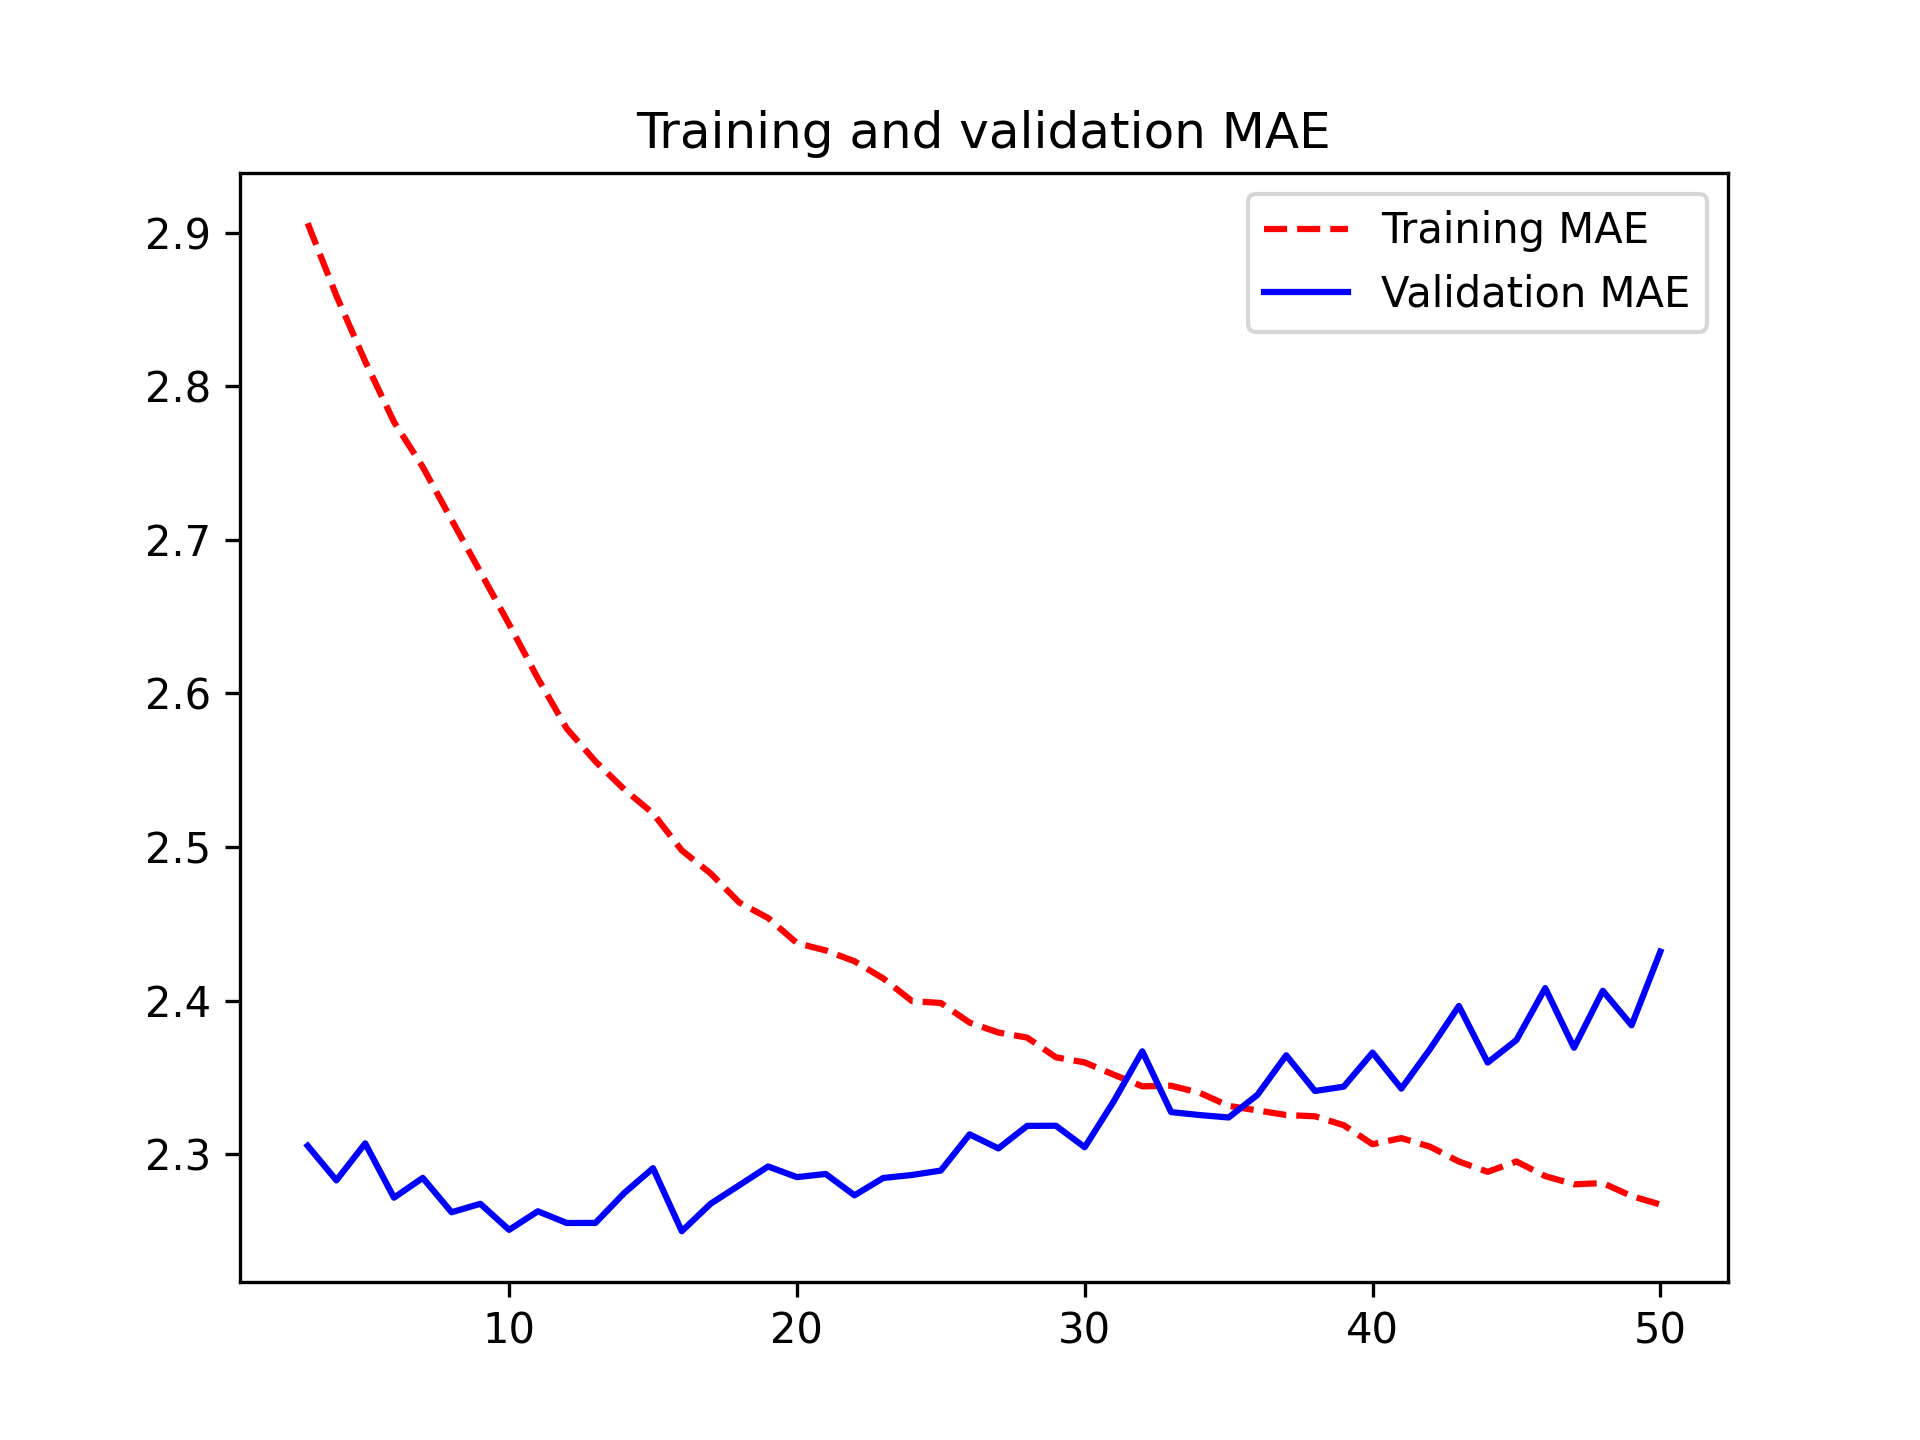
\includegraphics[width=\textwidth,height=0.6\textheight,keepaspectratio]{../../images/ch13/stacked_gru_dropout_model_metrics.5bfbf251.png}
            \caption{Xếp chồng GRU + Dropout}
        \end{figure}
    \end{columns}
\end{frame}

\begin{frame}{Kỹ thuật 3: Mạng truyền hồi Hai chiều (Bidirectional RNN)}
    \begin{columns}
        \column{0.5\textwidth}
        \begin{itemize}
            \item RNN thông thường chỉ đọc dữ liệu theo chiều thời gian (Từ quá khứ tới hiện tại).
            \item Bidirectional RNN dùng 2 lớp RNN độc lập: 1 đọc xuôi, 1 đọc ngược (từ tương lai về quá khứ), sau đó gộp kết quả lại.
            \item Vô cùng hữu ích trong xử lý ngôn ngữ tự nhiên (NLP) khi ý nghĩa của một từ phụ thuộc vào những từ phía sau nó.
        \end{itemize}
        
        \column{0.5\textwidth}
        \begin{figure}
            \centering
            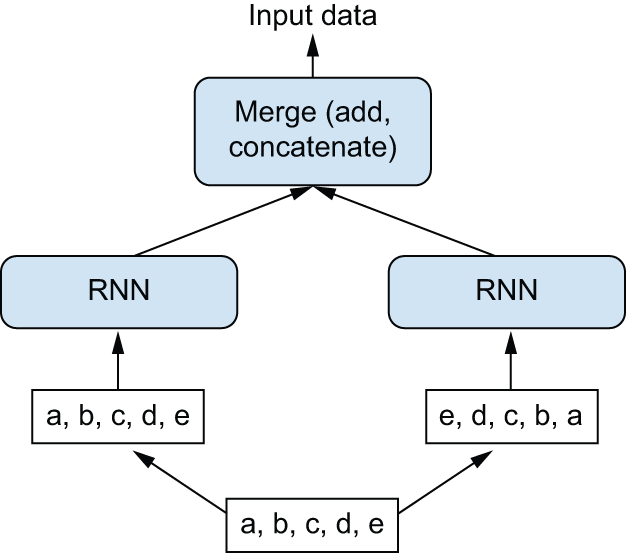
\includegraphics[width=\textwidth,height=0.5\textheight,keepaspectratio]{../../images/ch13/bidirectional_rnn.a38aaba4.png}
            \caption{Kiến trúc Bidirectional RNN}
        \end{figure}
    \end{columns}
\end{frame}

\begin{frame}[fragile]{Xây dựng Bidirectional LSTM}
Lớp \texttt{Bidirectional} của Keras đóng vai trò như một wrapper, nhân đôi LSTM bên trong nó và đảo ngược chuỗi thời gian cho nhân bản thứ hai.
\begin{lstlisting}[language=Python]
inputs = keras.Input(shape=(sequence_length, raw_data.shape[-1]))

# Wrap the LSTM layer inside a Bidirectional wrapper
x = layers.Bidirectional(layers.LSTM(16))(inputs)

outputs = layers.Dense(1)(x)
model = keras.Model(inputs, outputs)

model.compile(optimizer="adam", loss="mse", metrics=["mae"])
\end{lstlisting}
\textit{Tuy nhiên, Bidirectional hoạt động rất kém trên tập dữ liệu Thời tiết, bởi vì yếu tố quá khứ đóng vai trò quan trọng, trong khi chiều đọc ngược (tương lai về quá khứ) chứa dữ liệu gây nhiễu loạn luồng Logic của LSTM.}
\end{frame}

\section{Tổng kết}

\begin{frame}{Tổng kết Chương 13}
    \begin{itemize}
        \item \textbf{Timeseries (Chuỗi thời gian)} khác biệt hoàn toàn với dữ liệu thông thường vì thứ tự cấu thành nên ý nghĩa. Dense và Conv1D không phù hợp.
        \item \textbf{Mạng truyền hồi (RNN)} duy trì "Trạng thái" bộ nhớ, nhưng vướng phải lỗi Triệt tiêu đạo hàm (Vanishing Gradients).
        \item \textbf{LSTM / GRU} giải quyết triệt để lỗi trên bằng hệ thống Cổng (Gates) và Trạng thái Tế bào (Cell State $C_t$).
        \item Các kĩ thuật nâng cao như \textbf{Recurrent Dropout}, \textbf{Stacked RNN}, và \textbf{Bidirectional RNN} giúp tối ưu hóa hiệu suất tối đa.
    \end{itemize}
\end{frame}

\end{document}
